%%%%%%%%%%%%%%%%%%%%%%%%%%%%%%%%%%%%%%%%%%%%%%%%%%%%%%%%%%%%%%%%%%%
%                                                                 %
%   CERNLIB -- Short write ups -- LaTeX Source                    %
%                                                                 %
%   Front Material: Title page,                                   %
%                   Copyright Notice                              %
%                   Preliminary Remarks                           %
%                   Table of Contents                             %
%   EPS file      : cern15.eps, cnastit.eps                       %
%                                                                 %
%   Editor: Michel Goossens / CN-AS                               %
%   Last Mod.: 14 Nov  1994 16:30 mg                              %
%                                                                 %
%%%%%%%%%%%%%%%%%%%%%%%%%%%%%%%%%%%%%%%%%%%%%%%%%%%%%%%%%%%%%%%%%%%
 
%%%%%%%%%%%%%%%%%%%%%%%%%%%%%%%%%%%%%%%%%%%%%%%%%%%%%%%%%%%%%%%%%%%%
%    Tile page                                                     %
%%%%%%%%%%%%%%%%%%%%%%%%%%%%%%%%%%%%%%%%%%%%%%%%%%%%%%%%%%%%%%%%%%%%
%\def\Ptitle#1{\special{ps: /Printstring (#1) def}
%\epsfbox{cnastit.eps}}
 
\begin{titlepage}
\vspace*{-23mm}
\mbox{\resizebox{!}{30mm}{\includegraphics{cern15.eps}}}
\hfill
\raise8mm\hbox{\huge\bf CERN Program Library}
\hfill\mbox{}
\begin{center}
\mbox{}\\[10mm]
\mbox{\Ptitle{CERNLIB}}\\[3cm]
{\Huge Short Writeups}\\[5cm]
%{\LARGE Version---   June 1995}\\[4cm]
{\LARGE Application Software and Databases}\\[1cm]
{\LARGE Computing and Networks Division}\\[2cm]
\end{center}
\vfill
\begin{center}\Large CERN Geneva, Switzerland\end{center}
\end{titlepage}
 
%%%%%%%%%%%%%%%%%%%%%%%%%%%%%%%%%%%%%%%%%%%%%%%%%%%%%%%%%%%%%%%%%%%%
%    Copyright  page                                               %
%%%%%%%%%%%%%%%%%%%%%%%%%%%%%%%%%%%%%%%%%%%%%%%%%%%%%%%%%%%%%%%%%%%%
\thispagestyle{empty}
\framebox[\textwidth][t]{\hfill\begin{minipage}{0.96\textwidth}%
\vspace*{3mm}\begin{center}Copyright Notice\end{center}
\parskip\baselineskip
{\bf CERNLIB -- CERN Program Library Short writeups}
 
\copyright{} Copyright CERN, Geneva 1996
 
Copyright and any other appropriate legal protection of these
computer programs and associated documentation reserved in all
countries of the world.
 
These programs or documentation may not be reproduced by any
method without prior written consent of the Director-General
of CERN or his delegate.
 
Permission for the usage of any programs described herein is
granted apriori to those scientific institutes associated with
the CERN experimental program or with whom CERN has concluded
a scientific collaboration agreement.
 
CERN welcomes comments concerning the Program Library,
but undertakes no obligation for the maintenance of the programs,
nor responsibility for their correctness, and accepts no liability
whatsoever resulting from the use of its programs.
 
Requests for information should be addressed to:
\vspace*{-.5\baselineskip}
\begin{center}
\tt\begin{tabular}{l}
CERN Program Library Office              \\
CERN-CN Division                         \\
CH-1211 Geneva 23                        \\
Switzerland                              \\
Tel.      +41 22 767 4951                \\
Fax.      +41 22 767 8630                \\
Internet: cernlib@cern.ch
\end{tabular}
\end{center}
\vspace*{2mm}
\end{minipage}\hfill}%end of minipage in framebox
\vspace{6mm}
 
{\bf Trademark notice: All trademarks appearing in this guide are acknowledged as such.}
\vfill
\begin{tabular}{l@{\qquad}l@{\quad}>{\tt}l}
{\em Contact Person\/}:        & Jamie Shiers /CN & (shiers\atsign cern.ch)\\[1mm]
{\em Technical Realization\/}: & Michel Goossens /CN & (goossens\atsign cern.ch)\\[1cm]
{\em Edition -- June 1996}
\end{tabular}
\newpage
 
%%%%%%%%%%%%%%%%%%%%%%%%%%%%%%%%%%%%%%%%%%%%%%%%%%%%%%%%%%%%%%%%%%%%
%    Introductory material                                         %
%%%%%%%%%%%%%%%%%%%%%%%%%%%%%%%%%%%%%%%%%%%%%%%%%%%%%%%%%%%%%%%%%%%%
\def\Rtnr{Front} % Dummy routine name to appear at bottom of page
\pagenumbering{roman}
\setcounter{page}{1}
 
\section*{Introduction}
 
The CERN Program Library is a large collection of general-purpose
programs maintained and offered in both source and object code form on
the CERN central computers. Most of these programs were developed at
CERN and are therefore oriented towards the needs of a physics
research laboratory.  Nearly all, however, are of a general
mathematical or data-handling nature, applicable to a wide range of
problems.
 
The library is heavily used at CERN and it is distributed in binary or
source form to several hundred laboratories and computer centres
outside CERN.
 
\subsection*{Contents and Organization of the Library}
 
The library contains about 2500 subroutines and complete programs
which are grouped together by logical affiliation into little over 450
program packages.  80\% of the programs are written in Fortran77 and
the remainder in C and in assembly code, usually with a FORTRAN
version also available.
 
A unique code is assigned to each package.  This code consists of one
letter and three or four digits, the letter indicating the category
within our classification scheme.  A package consists of one or more
related subprograms with one package name and one or more
user-callable entry names, all described briefly in a ``Short
write-up'', and if necessary, an additional ``Long write-up''.
 
A complete list of program packages with titles and entries sorted by
class is given at the beginning of this manual.  Then follow all the
short write-ups, while the Index at the end of the volume shows the
page number (as printed near the inner margin) were a package is
defined (in {\bf boldface}) or referenced.
 
\subsection*{Acknowledgements}
 
K.S.~K\"olbig has done most of the work for having this manual nicely
formated, particularly in the area of getting the many mathematical
formulae correct.
 
\subsection*{About the documentation}
 
This document has been produced using \LaTeX\footnote{%
  Leslie Lamport, \textem{\LaTeX\ -- A Document Preparation System},
  second edition. Addison--Wesley, 1994} 
with the \Lit{cernman} class
and the \Lit{cernlib} package, developed at CERN.  A printable version
of each of the routines described in this manual can be obtained as a
compressed PostScript file from CERN by anonymous ftp. For instance,
if you want to transfer the description of routine E112, then you
would type the following (commands that you have to type are
underlined):\footnote{You can of course issue multiple \Ucom{get}
  commands in one run.  If you do not have the \Lit{gunzip} utility on
  your machine, you can get an non-compressed, ready-to-print version
  by omitting the \Lit{.gz} suffix, i.e.\ in the example above,
  \Ucom{get e112.ps}.} 
\vspace*{3mm}
\begin{tabular}{@{\hspace{12mm}}>{\tt}l}
\Ucom{ftp asisftp.cern.ch}\\
Trying 128.141.201.136...\\
Connected to asis01.cern.ch.\\
220 asis01 FTP server (SunOS 4.1) ready.\\
Name (asis01:username): \Ucom{anonymous}\\
Password: \Ucom{your\_{}mailaddress}\\
ftp> \Ucom{binary}        \\
ftp> \Ucom{cd cernlib/doc/ps.dir/shortwrups.dir}\\
ftp> \Ucom{get e112.ps.gz} \\
ftp> \Ucom{quit}        
\end{tabular}
